%!TEX program = lualatex
% SPDX-License-Identifier: CC-BY-SA-4.0
\documentclass[11pt]{article}

\usepackage{iftex}
\ifLuaTeX\else
  \PackageError{vintage-latex}{This example requires LuaLaTeX}
    {Run lualatex, not pdflatex or xelatex.}
\fi

\usepackage{fontspec}
\usepackage{xcolor}
\usepackage{geometry}
\usepackage[tracking=true,protrusion=false,expansion=false]{microtype}
\usepackage{tikz}
\usetikzlibrary{calc}

\defaultfontfeatures{Renderer=HarfBuzz}
\setmainfont{EB Garamond}[Numbers={OldStyle,Proportional}]
\definecolor{chartpaper}{HTML}{F3E9D6}
\definecolor{printerink}{HTML}{25201B}
\definecolor{gridink}{HTML}{7A6A55}
\pagecolor{chartpaper}
\color{printerink}
\geometry{a4paper,top=20mm,bottom=20mm,left=24mm,right=24mm}
\pagestyle{empty}

% Polar projection about the north celestial pole. Right ascension becomes the
% polar angle and the distance from the pole grows with 90 - declination, so
% the chart reads correctly when held overhead.
\newcommand{\chartradius}{7.2}   % radius of the +35 degree limit, in cm
\newcommand{\declimit}{35}
\newcommand{\starpos}[2]{% #1 = RA in hours, #2 = declination in degrees
  ({15*#1}:{\chartradius*(90-#2)/(90-\declimit)})}

\begin{document}

\begin{center}
  {\small\textls[120]{\textsc{Plate IV}}}\par
  \vspace{.3em}
  {\Large The Circumpolar Stars}\par
  \vspace{.2em}
  {\itshape as seen from latitude 52\textdegree\ north; the pole at the centre}
\end{center}

\vspace{.4em}

\begin{center}
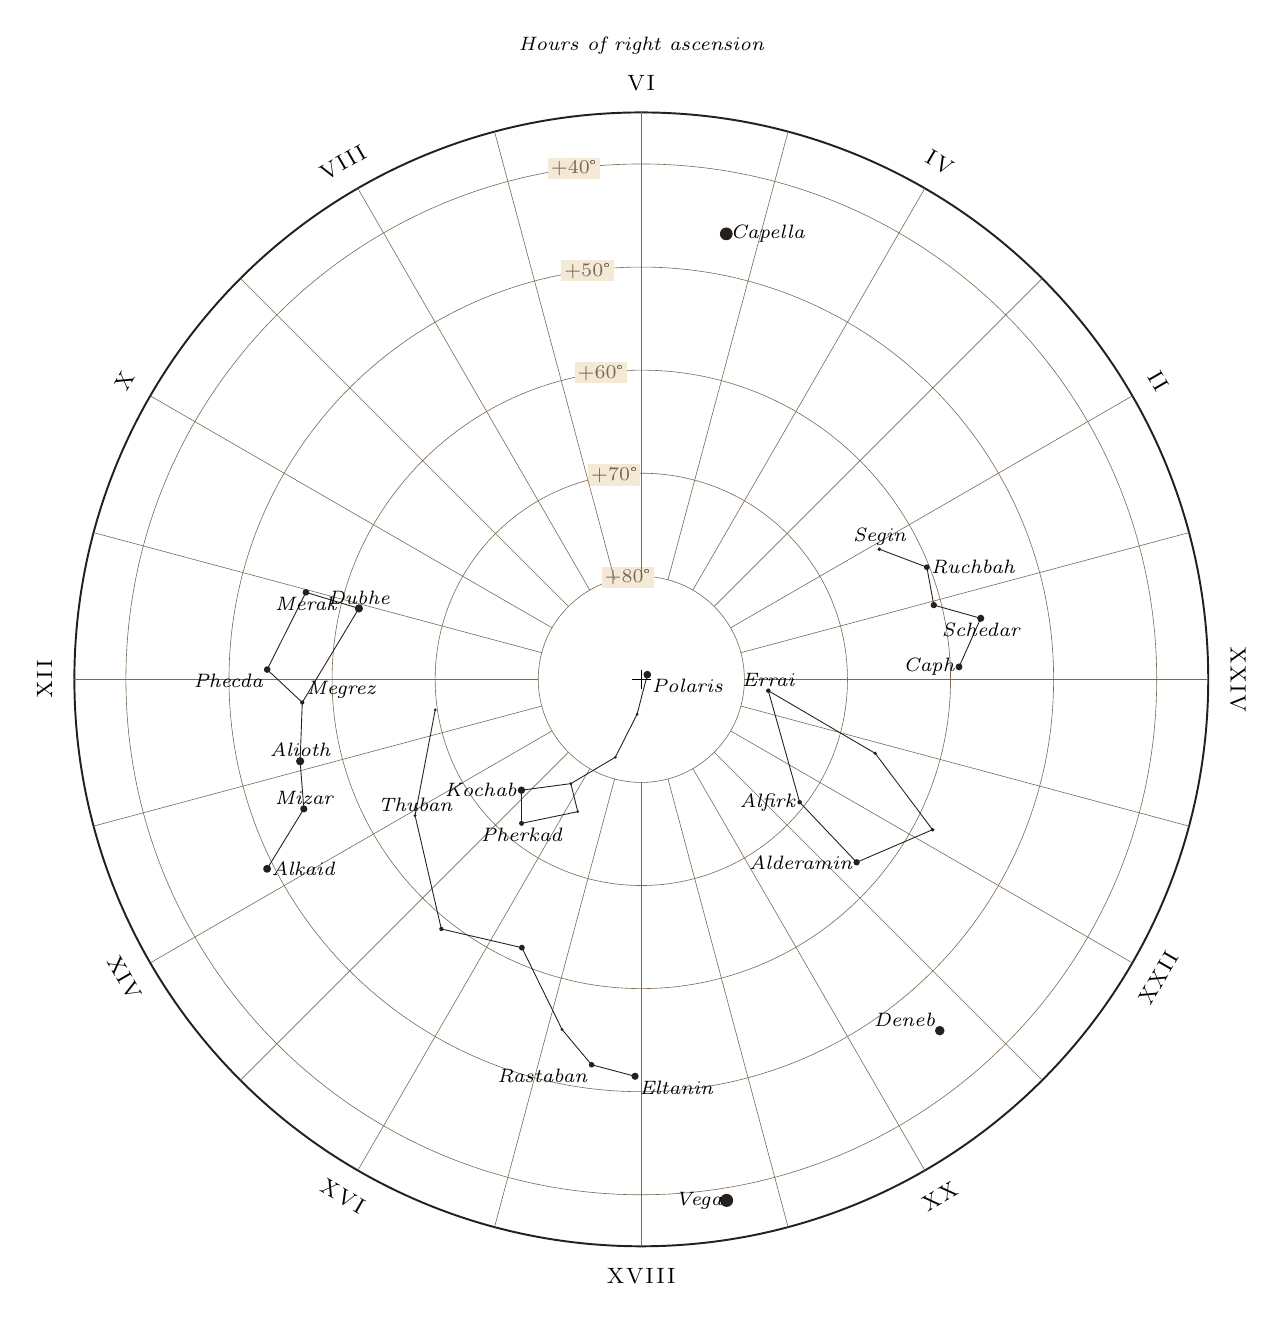
\begin{tikzpicture}[x=1cm,y=1cm]
  % Declination circles, every ten degrees from the pole to the chart limit.
  \foreach \dec in {80,70,...,40} {
    \draw[gridink,line width=.22pt]
      (0,0) circle[radius={\chartradius*(90-\dec)/(90-\declimit)}];
    \node[gridink,font=\scriptsize,fill=chartpaper,inner sep=1pt]
      at ({15*6.5}:{\chartradius*(90-\dec)/(90-\declimit)}) {+\dec\textdegree};
  }
  \draw[printerink,line width=.7pt] (0,0) circle[radius=\chartradius];

  % Hour circles of right ascension, labelled in roman numerals on the rim.
  \foreach \h [evaluate=\h as \ang using 15*\h] in {0,1,...,23} {
    \draw[gridink,line width=.22pt]
      (\ang:{\chartradius*10/(90-\declimit)}) -- (\ang:\chartradius);
  }
  % Rim numerals stay upright: those on the lower half are turned the other way.
  \foreach \h/\rn in {0/XXIV,2/II,4/IV,6/VI,8/VIII,10/X,12/XII,14/XIV,
                      16/XVI,18/XVIII,20/XX,22/XXII} {
    \pgfmathsetmacro{\turn}{ifthenelse(15*\h>180, 15*\h+90, 15*\h-90)}
    \node[font=\footnotesize\scshape,rotate=\turn]
      at ({15*\h}:{\chartradius+.38}) {\rn};
  }
  \node[font=\scriptsize\itshape] at (90:{\chartradius+.85})
    {Hours of right ascension};

  % Constellation figures: joined star to star, as on the old planispheres.
  \begin{scope}[printerink,line width=.32pt]
    % Ursa Major, the Plough.
    \draw \starpos{11.06}{61.75} -- \starpos{11.03}{56.38}
       -- \starpos{11.90}{53.69} -- \starpos{12.26}{57.03}
       -- \starpos{11.06}{61.75};
    \draw \starpos{12.26}{57.03} -- \starpos{12.90}{55.96}
       -- \starpos{13.40}{54.93} -- \starpos{13.79}{49.31};
    % Ursa Minor, from Polaris to the bowl.
    \draw \starpos{2.53}{89.26} -- \starpos{17.54}{86.59}
       -- \starpos{16.77}{82.04} -- \starpos{15.73}{77.79}
       -- \starpos{14.85}{74.16} -- \starpos{15.35}{71.83}
       -- \starpos{16.29}{75.76} -- \starpos{15.73}{77.79};
    % Cassiopeia, the W.
    \draw \starpos{0.15}{59.15} -- \starpos{0.68}{56.54}
       -- \starpos{0.95}{60.72} -- \starpos{1.43}{60.24}
       -- \starpos{1.91}{63.67};
    % Cepheus, the house.
    \draw \starpos{21.31}{62.59} -- \starpos{21.48}{70.56}
       -- \starpos{23.66}{77.63} -- \starpos{22.83}{66.20}
       -- \starpos{22.18}{58.20} -- \starpos{21.31}{62.59};
    % Draco, the head and part of the body.
    \draw \starpos{17.94}{51.49} -- \starpos{17.51}{52.30}
       -- \starpos{17.15}{55.17} -- \starpos{16.40}{61.51}
       -- \starpos{15.42}{58.97} -- \starpos{14.07}{64.38}
       -- \starpos{12.56}{69.79};
  \end{scope}

  % Stars. Disc radius follows magnitude, as engravers graded their stars.
  \foreach \ra/\dec/\mag/\name/\pos in {
    2.53/89.26/2.0/Polaris/below right,
    11.06/61.75/1.8/Dubhe/above,
    11.03/56.38/2.4/Merak/below,
    11.90/53.69/2.4/Phecda/below left,
    12.26/57.03/3.3/Megrez/above right,
    12.90/55.96/1.8/Alioth/above,
    13.40/54.93/2.2/Mizar/above,
    13.79/49.31/1.9/Alkaid/right,
    14.85/74.16/2.1/Kochab/left,
    15.35/71.83/3.0/Pherkad/below,
    17.54/86.59/4.4//,
    16.77/82.04/4.3//,
    15.73/77.79/4.2//,
    16.29/75.76/5.0//,
    0.15/59.15/2.3/Caph/left,
    0.68/56.54/2.2/Schedar/below,
    0.95/60.72/2.5//,
    1.43/60.24/2.7/Ruchbah/right,
    1.91/63.67/3.4/Segin/above,
    5.28/46.00/0.1/Capella/right,
    18.62/38.78/0.0/Vega/left,
    20.69/45.28/1.3/Deneb/above left,
    21.31/62.59/2.5/Alderamin/left,
    21.48/70.56/3.2/Alfirk/left,
    23.66/77.63/3.2/Errai/above,
    22.83/66.20/3.5//,
    22.18/58.20/3.4//,
    17.94/51.49/2.2/Eltanin/below right,
    17.51/52.30/2.8/Rastaban/below left,
    17.15/55.17/3.7//,
    16.40/61.51/2.7//,
    15.42/58.97/3.3//,
    14.07/64.38/3.7/Thuban/above,
    12.56/69.79/3.8//} {
    \pgfmathsetmacro{\starr}{max(0.55, 2.35-0.48*\mag)}
    \fill[printerink] \starpos{\ra}{\dec} circle[radius=\starr pt];
    \ifx\name\empty\else
      \node[font=\scriptsize\itshape,\pos,inner sep=1.4pt]
        at \starpos{\ra}{\dec} {\name};
    \fi
  }

  % Small cross at the pole, distinct from Polaris a little way off.
  \draw[line width=.35pt] (-.12,0)--(.12,0) (0,-.12)--(0,.12);
\end{tikzpicture}
\end{center}

\vspace{.5em}
\begin{center}
\small
\begin{tabular}{@{}c@{\hspace{1.4em}}c@{\hspace{1.4em}}c@{\hspace{1.4em}}c@{\hspace{1.4em}}c@{}}
  \tikz\fill (0,0) circle[radius=2.35pt]; &
  \tikz\fill (0,0) circle[radius=1.87pt]; &
  \tikz\fill (0,0) circle[radius=1.39pt]; &
  \tikz\fill (0,0) circle[radius=0.91pt]; &
  \tikz\fill (0,0) circle[radius=0.55pt];\\
  1st mag. & 2nd & 3rd & 4th & 5th
\end{tabular}
\end{center}

\vspace{.4em}
\footnotesize\noindent
Positions are rounded epoch-2000 coordinates of thirty-four naked-eye stars.
Every star, grid line, and label is placed by one macro that converts right
ascension and declination to polar coordinates, so the same source can be
re-centred, re-limited, or extended with further stars without redrawing.

\end{document}
